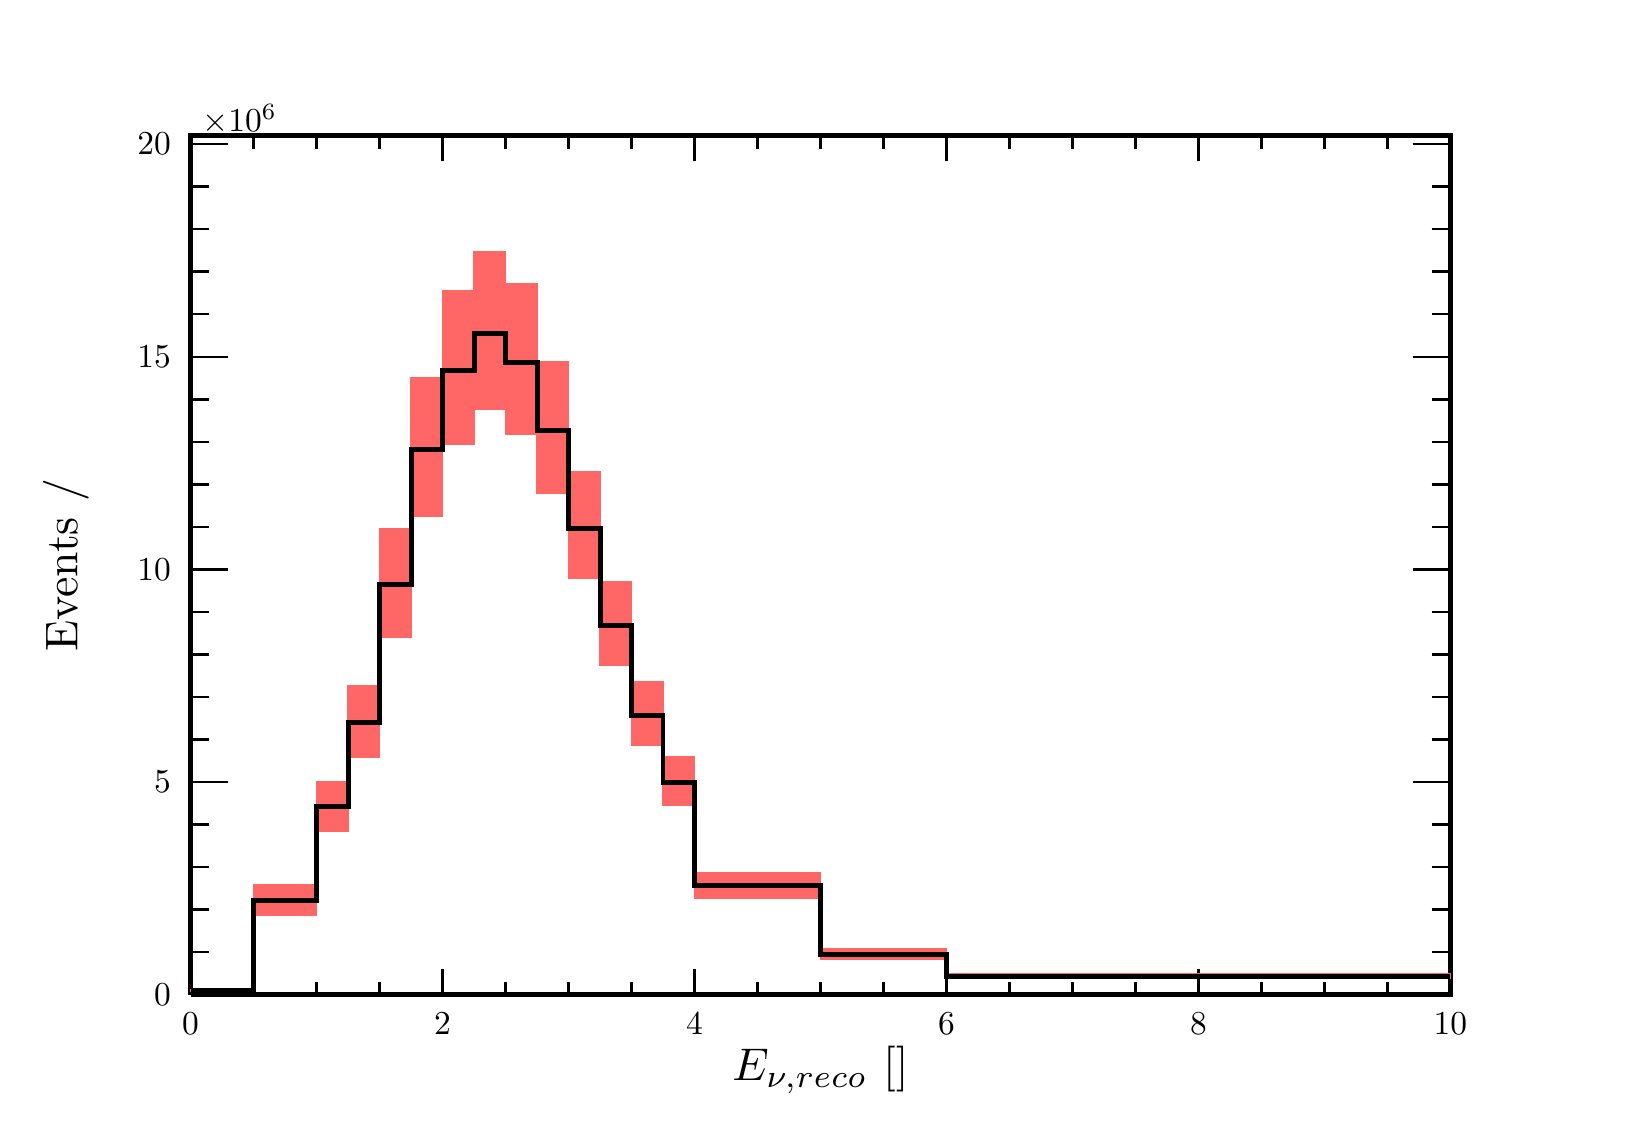
\begin{tikzpicture}
\pgfdeclareplotmark{cross} {
\pgfpathmoveto{\pgfpoint{-0.3\pgfplotmarksize}{\pgfplotmarksize}}
\pgfpathlineto{\pgfpoint{+0.3\pgfplotmarksize}{\pgfplotmarksize}}
\pgfpathlineto{\pgfpoint{+0.3\pgfplotmarksize}{0.3\pgfplotmarksize}}
\pgfpathlineto{\pgfpoint{+1\pgfplotmarksize}{0.3\pgfplotmarksize}}
\pgfpathlineto{\pgfpoint{+1\pgfplotmarksize}{-0.3\pgfplotmarksize}}
\pgfpathlineto{\pgfpoint{+0.3\pgfplotmarksize}{-0.3\pgfplotmarksize}}
\pgfpathlineto{\pgfpoint{+0.3\pgfplotmarksize}{-1.\pgfplotmarksize}}
\pgfpathlineto{\pgfpoint{-0.3\pgfplotmarksize}{-1.\pgfplotmarksize}}
\pgfpathlineto{\pgfpoint{-0.3\pgfplotmarksize}{-0.3\pgfplotmarksize}}
\pgfpathlineto{\pgfpoint{-1.\pgfplotmarksize}{-0.3\pgfplotmarksize}}
\pgfpathlineto{\pgfpoint{-1.\pgfplotmarksize}{0.3\pgfplotmarksize}}
\pgfpathlineto{\pgfpoint{-0.3\pgfplotmarksize}{0.3\pgfplotmarksize}}
\pgfpathclose
\pgfusepathqstroke
}
\pgfdeclareplotmark{cross*} {
\pgfpathmoveto{\pgfpoint{-0.3\pgfplotmarksize}{\pgfplotmarksize}}
\pgfpathlineto{\pgfpoint{+0.3\pgfplotmarksize}{\pgfplotmarksize}}
\pgfpathlineto{\pgfpoint{+0.3\pgfplotmarksize}{0.3\pgfplotmarksize}}
\pgfpathlineto{\pgfpoint{+1\pgfplotmarksize}{0.3\pgfplotmarksize}}
\pgfpathlineto{\pgfpoint{+1\pgfplotmarksize}{-0.3\pgfplotmarksize}}
\pgfpathlineto{\pgfpoint{+0.3\pgfplotmarksize}{-0.3\pgfplotmarksize}}
\pgfpathlineto{\pgfpoint{+0.3\pgfplotmarksize}{-1.\pgfplotmarksize}}
\pgfpathlineto{\pgfpoint{-0.3\pgfplotmarksize}{-1.\pgfplotmarksize}}
\pgfpathlineto{\pgfpoint{-0.3\pgfplotmarksize}{-0.3\pgfplotmarksize}}
\pgfpathlineto{\pgfpoint{-1.\pgfplotmarksize}{-0.3\pgfplotmarksize}}
\pgfpathlineto{\pgfpoint{-1.\pgfplotmarksize}{0.3\pgfplotmarksize}}
\pgfpathlineto{\pgfpoint{-0.3\pgfplotmarksize}{0.3\pgfplotmarksize}}
\pgfpathclose
\pgfusepathqfillstroke
}
\pgfdeclareplotmark{newstar} {
\pgfpathmoveto{\pgfqpoint{0pt}{\pgfplotmarksize}}
\pgfpathlineto{\pgfqpointpolar{44}{0.5\pgfplotmarksize}}
\pgfpathlineto{\pgfqpointpolar{18}{\pgfplotmarksize}}
\pgfpathlineto{\pgfqpointpolar{-20}{0.5\pgfplotmarksize}}
\pgfpathlineto{\pgfqpointpolar{-54}{\pgfplotmarksize}}
\pgfpathlineto{\pgfqpointpolar{-90}{0.5\pgfplotmarksize}}
\pgfpathlineto{\pgfqpointpolar{234}{\pgfplotmarksize}}
\pgfpathlineto{\pgfqpointpolar{198}{0.5\pgfplotmarksize}}
\pgfpathlineto{\pgfqpointpolar{162}{\pgfplotmarksize}}
\pgfpathlineto{\pgfqpointpolar{134}{0.5\pgfplotmarksize}}
\pgfpathclose
\pgfusepathqstroke
}
\pgfdeclareplotmark{newstar*} {
\pgfpathmoveto{\pgfqpoint{0pt}{\pgfplotmarksize}}
\pgfpathlineto{\pgfqpointpolar{44}{0.5\pgfplotmarksize}}
\pgfpathlineto{\pgfqpointpolar{18}{\pgfplotmarksize}}
\pgfpathlineto{\pgfqpointpolar{-20}{0.5\pgfplotmarksize}}
\pgfpathlineto{\pgfqpointpolar{-54}{\pgfplotmarksize}}
\pgfpathlineto{\pgfqpointpolar{-90}{0.5\pgfplotmarksize}}
\pgfpathlineto{\pgfqpointpolar{234}{\pgfplotmarksize}}
\pgfpathlineto{\pgfqpointpolar{198}{0.5\pgfplotmarksize}}
\pgfpathlineto{\pgfqpointpolar{162}{\pgfplotmarksize}}
\pgfpathlineto{\pgfqpointpolar{134}{0.5\pgfplotmarksize}}
\pgfpathclose
\pgfusepathqfillstroke
}
\definecolor{c}{rgb}{0.999,0.999,0.999};
\draw [color=c, fill=c] (0,0) rectangle (20,13.639);
\draw [color=c, fill=c] (2,1.3639) rectangle (18,12.2751);
\definecolor{c}{rgb}{0,0,0};
\draw [c,line width=1.8] (2,1.3639) -- (2,12.2751) -- (18,12.2751) -- (18,1.3639) -- (2,1.3639);
\definecolor{c}{rgb}{0.999,0.999,0.999};
\draw [color=c, fill=c] (2,1.3639) rectangle (18,12.2751);
\definecolor{c}{rgb}{0,0,0};
\draw [c,line width=1.8] (2,1.3639) -- (2,12.2751) -- (18,12.2751) -- (18,1.3639) -- (2,1.3639);
\draw [c,line width=1.8] (2,1.41404) -- (2.8,1.41404) -- (2.8,2.55873) -- (3.6,2.55873) -- (3.6,3.75039) -- (4,3.75039) -- (4,4.82314) -- (4.4,4.82314) -- (4.4,6.57373) -- (4.8,6.57373) -- (4.8,8.28708) -- (5.2,8.28708) -- (5.2,9.29376) --
 (5.6,9.29376) -- (5.6,9.75711) -- (6,9.75711) -- (6,9.39589) -- (6.4,9.39589) -- (6.4,8.52387) -- (6.8,8.52387) -- (6.8,7.29096) -- (7.2,7.29096) -- (7.2,6.04917) -- (7.6,6.04917) -- (7.6,4.91319) -- (8,4.91319) -- (8,4.06482) -- (8.4,4.06482) --
 (8.4,2.74593) -- (10,2.74593) -- (10,1.87667) -- (11.6,1.87667) -- (11.6,1.59709) -- (18,1.59709);
\draw [c,line width=0.9] (2,1.3639) -- (18,1.3639);
\draw [c,line width=0.9] (2,1.69123) -- (2,1.3639);
\draw [c,line width=0.9] (2.8,1.52756) -- (2.8,1.3639);
\draw [c,line width=0.9] (3.6,1.52756) -- (3.6,1.3639);
\draw [c,line width=0.9] (4.4,1.52756) -- (4.4,1.3639);
\draw [c,line width=0.9] (5.2,1.69123) -- (5.2,1.3639);
\draw [c,line width=0.9] (6,1.52756) -- (6,1.3639);
\draw [c,line width=0.9] (6.8,1.52756) -- (6.8,1.3639);
\draw [c,line width=0.9] (7.6,1.52756) -- (7.6,1.3639);
\draw [c,line width=0.9] (8.4,1.69123) -- (8.4,1.3639);
\draw [c,line width=0.9] (9.2,1.52756) -- (9.2,1.3639);
\draw [c,line width=0.9] (10,1.52756) -- (10,1.3639);
\draw [c,line width=0.9] (10.8,1.52756) -- (10.8,1.3639);
\draw [c,line width=0.9] (11.6,1.69123) -- (11.6,1.3639);
\draw [c,line width=0.9] (12.4,1.52756) -- (12.4,1.3639);
\draw [c,line width=0.9] (13.2,1.52756) -- (13.2,1.3639);
\draw [c,line width=0.9] (14,1.52756) -- (14,1.3639);
\draw [c,line width=0.9] (14.8,1.69123) -- (14.8,1.3639);
\draw [c,line width=0.9] (15.6,1.52756) -- (15.6,1.3639);
\draw [c,line width=0.9] (16.4,1.52756) -- (16.4,1.3639);
\draw [c,line width=0.9] (17.2,1.52756) -- (17.2,1.3639);
\draw [c,line width=0.9] (18,1.69123) -- (18,1.3639);
\draw [anchor=base] (2,0.859255) node[scale=1.20912, color=c, rotate=0]{0};
\draw [anchor=base] (5.2,0.859255) node[scale=1.20912, color=c, rotate=0]{2};
\draw [anchor=base] (8.4,0.859255) node[scale=1.20912, color=c, rotate=0]{4};
\draw [anchor=base] (11.6,0.859255) node[scale=1.20912, color=c, rotate=0]{6};
\draw [anchor=base] (14.8,0.859255) node[scale=1.20912, color=c, rotate=0]{8};
\draw [anchor=base] (18,0.859255) node[scale=1.20912, color=c, rotate=0]{10};
\draw (10,0.403714) node[scale=1.65459, color=c, rotate=0]{$E_{\nu, \text{reco}}$ [\si{\GeV}]};
\draw [c,line width=0.9] (2,12.2751) -- (18,12.2751);
\draw [c,line width=0.9] (2,11.9477) -- (2,12.2751);
\draw [c,line width=0.9] (2.8,12.1114) -- (2.8,12.2751);
\draw [c,line width=0.9] (3.6,12.1114) -- (3.6,12.2751);
\draw [c,line width=0.9] (4.4,12.1114) -- (4.4,12.2751);
\draw [c,line width=0.9] (5.2,11.9477) -- (5.2,12.2751);
\draw [c,line width=0.9] (6,12.1114) -- (6,12.2751);
\draw [c,line width=0.9] (6.8,12.1114) -- (6.8,12.2751);
\draw [c,line width=0.9] (7.6,12.1114) -- (7.6,12.2751);
\draw [c,line width=0.9] (8.4,11.9477) -- (8.4,12.2751);
\draw [c,line width=0.9] (9.2,12.1114) -- (9.2,12.2751);
\draw [c,line width=0.9] (10,12.1114) -- (10,12.2751);
\draw [c,line width=0.9] (10.8,12.1114) -- (10.8,12.2751);
\draw [c,line width=0.9] (11.6,11.9477) -- (11.6,12.2751);
\draw [c,line width=0.9] (12.4,12.1114) -- (12.4,12.2751);
\draw [c,line width=0.9] (13.2,12.1114) -- (13.2,12.2751);
\draw [c,line width=0.9] (14,12.1114) -- (14,12.2751);
\draw [c,line width=0.9] (14.8,11.9477) -- (14.8,12.2751);
\draw [c,line width=0.9] (15.6,12.1114) -- (15.6,12.2751);
\draw [c,line width=0.9] (16.4,12.1114) -- (16.4,12.2751);
\draw [c,line width=0.9] (17.2,12.1114) -- (17.2,12.2751);
\draw [c,line width=0.9] (18,11.9477) -- (18,12.2751);
\draw [c,line width=0.9] (2,1.3639) -- (2,12.2751);
\draw [c,line width=0.9] (2.48,1.3639) -- (2,1.3639);
\draw [c,line width=0.9] (2.24,1.90408) -- (2,1.90408);
\draw [c,line width=0.9] (2.24,2.44427) -- (2,2.44427);
\draw [c,line width=0.9] (2.24,2.98445) -- (2,2.98445);
\draw [c,line width=0.9] (2.24,3.52464) -- (2,3.52464);
\draw [c,line width=0.9] (2.48,4.06482) -- (2,4.06482);
\draw [c,line width=0.9] (2.24,4.60501) -- (2,4.60501);
\draw [c,line width=0.9] (2.24,5.14519) -- (2,5.14519);
\draw [c,line width=0.9] (2.24,5.68538) -- (2,5.68538);
\draw [c,line width=0.9] (2.24,6.22556) -- (2,6.22556);
\draw [c,line width=0.9] (2.48,6.76575) -- (2,6.76575);
\draw [c,line width=0.9] (2.24,7.30593) -- (2,7.30593);
\draw [c,line width=0.9] (2.24,7.84612) -- (2,7.84612);
\draw [c,line width=0.9] (2.24,8.3863) -- (2,8.3863);
\draw [c,line width=0.9] (2.24,8.92649) -- (2,8.92649);
\draw [c,line width=0.9] (2.48,9.46667) -- (2,9.46667);
\draw [c,line width=0.9] (2.24,10.0069) -- (2,10.0069);
\draw [c,line width=0.9] (2.24,10.547) -- (2,10.547);
\draw [c,line width=0.9] (2.24,11.0872) -- (2,11.0872);
\draw [c,line width=0.9] (2.24,11.6274) -- (2,11.6274);
\draw [c,line width=0.9] (2.48,12.1676) -- (2,12.1676);
\draw [c,line width=0.9] (2.48,12.1676) -- (2,12.1676);
\draw [anchor= east] (1.9,1.3639) node[scale=1.20912, color=c, rotate=0]{0};
\draw [anchor= east] (1.9,4.06482) node[scale=1.20912, color=c, rotate=0]{5};
\draw [anchor= east] (1.9,6.76575) node[scale=1.20912, color=c, rotate=0]{10};
\draw [anchor= east] (1.9,9.46667) node[scale=1.20912, color=c, rotate=0]{15};
\draw [anchor= east] (1.9,12.1676) node[scale=1.20912, color=c, rotate=0]{20};
\draw [anchor=base west] (2,12.3296) node[scale=1.20912, color=c, rotate=0]{$\times10^{6}$};
\draw (0.416,6.81948) node[scale=1.65459, color=c, rotate=90]{Events / \si{\GeV}};
\draw [c,line width=0.9] (18,1.3639) -- (18,12.2751);
\draw [c,line width=0.9] (17.52,1.3639) -- (18,1.3639);
\draw [c,line width=0.9] (17.76,1.90408) -- (18,1.90408);
\draw [c,line width=0.9] (17.76,2.44427) -- (18,2.44427);
\draw [c,line width=0.9] (17.76,2.98445) -- (18,2.98445);
\draw [c,line width=0.9] (17.76,3.52464) -- (18,3.52464);
\draw [c,line width=0.9] (17.52,4.06482) -- (18,4.06482);
\draw [c,line width=0.9] (17.76,4.60501) -- (18,4.60501);
\draw [c,line width=0.9] (17.76,5.14519) -- (18,5.14519);
\draw [c,line width=0.9] (17.76,5.68538) -- (18,5.68538);
\draw [c,line width=0.9] (17.76,6.22556) -- (18,6.22556);
\draw [c,line width=0.9] (17.52,6.76575) -- (18,6.76575);
\draw [c,line width=0.9] (17.76,7.30593) -- (18,7.30593);
\draw [c,line width=0.9] (17.76,7.84612) -- (18,7.84612);
\draw [c,line width=0.9] (17.76,8.3863) -- (18,8.3863);
\draw [c,line width=0.9] (17.76,8.92649) -- (18,8.92649);
\draw [c,line width=0.9] (17.52,9.46667) -- (18,9.46667);
\draw [c,line width=0.9] (17.76,10.0069) -- (18,10.0069);
\draw [c,line width=0.9] (17.76,10.547) -- (18,10.547);
\draw [c,line width=0.9] (17.76,11.0872) -- (18,11.0872);
\draw [c,line width=0.9] (17.76,11.6274) -- (18,11.6274);
\draw [c,line width=0.9] (17.52,12.1676) -- (18,12.1676);
\draw [c,line width=0.9] (17.52,12.1676) -- (18,12.1676);
\definecolor{c}{rgb}{1,0.4,0.4};
\draw [color=c, fill=c] (2,1.40191) rectangle (2.8,1.42724);
\draw [color=c, fill=c] (2.8,2.37459) rectangle (3.6,2.75935);
\draw [color=c, fill=c] (3.6,3.44297) rectangle (4,4.07616);
\draw [color=c, fill=c] (4,4.37496) rectangle (4.4,5.29674);
\draw [color=c, fill=c] (4.4,5.90504) rectangle (4.8,7.28627);
\draw [color=c, fill=c] (4.8,7.43852) rectangle (5.2,9.19798);
\draw [color=c, fill=c] (5.2,8.35719) rectangle (5.6,10.3065);
\draw [color=c, fill=c] (5.6,8.79266) rectangle (6,10.8084);
\draw [color=c, fill=c] (6,8.48593) rectangle (6.4,10.3952);
\draw [color=c, fill=c] (6.4,7.73428) rectangle (6.8,9.39958);
\draw [color=c, fill=c] (6.8,6.64608) rectangle (7.2,8.0101);
\draw [color=c, fill=c] (7.2,5.54659) rectangle (7.6,6.61171);
\draw [color=c, fill=c] (7.6,4.53405) rectangle (8,5.33873);
\draw [color=c, fill=c] (8,3.77119) rectangle (8.4,4.39406);
\draw [color=c, fill=c] (8.4,2.5868) rectangle (10,2.9214);
\draw [color=c, fill=c] (10,1.81411) rectangle (11.6,1.94488);
\draw [color=c, fill=c] (11.6,1.56714) rectangle (18,1.62917);
\definecolor{c}{rgb}{0,0,0};
\draw [c,line width=1.8] (2,1.41404) -- (2.8,1.41404) -- (2.8,2.55873) -- (3.6,2.55873) -- (3.6,3.75039) -- (4,3.75039) -- (4,4.82314) -- (4.4,4.82314) -- (4.4,6.57373) -- (4.8,6.57373) -- (4.8,8.28708) -- (5.2,8.28708) -- (5.2,9.29376) --
 (5.6,9.29376) -- (5.6,9.75711) -- (6,9.75711) -- (6,9.39589) -- (6.4,9.39589) -- (6.4,8.52387) -- (6.8,8.52387) -- (6.8,7.29096) -- (7.2,7.29096) -- (7.2,6.04917) -- (7.6,6.04917) -- (7.6,4.91319) -- (8,4.91319) -- (8,4.06482) -- (8.4,4.06482) --
 (8.4,2.74593) -- (10,2.74593) -- (10,1.87667) -- (11.6,1.87667) -- (11.6,1.59709) -- (18,1.59709);
\end{tikzpicture}
